\section{UI}
Program UI~je~psaný v~jazyce C++ stejně jako program lasershow. Tento program ovládá OLED displej, který je~připojený na~Raspberry Pi~pomocí rozhraní I$^{2}$C, a~přijímá vstup od~uživatele čtením rotačního enkodéru s~tlačítkem. Také příjmá informace od~programů lasershow a~wifi\_manager a~posílá jim~vstup od~uživatele.

Na LCD~displeji má uživatel díky tomuto programu přístup k~menu, kde~jsou zobrazeny aktuální informace o~promítání a~wifi připojení a~kde uživatel může měnit nastavení dvou backendových programů. Fotky zobrazení menu jsou na obrázcích~\ref{fig:uilcdmain},~\ref{fig:uilcdsec} a~\ref{fig:uilcdwifi}.

\begin{figure}[H]
    \centering
    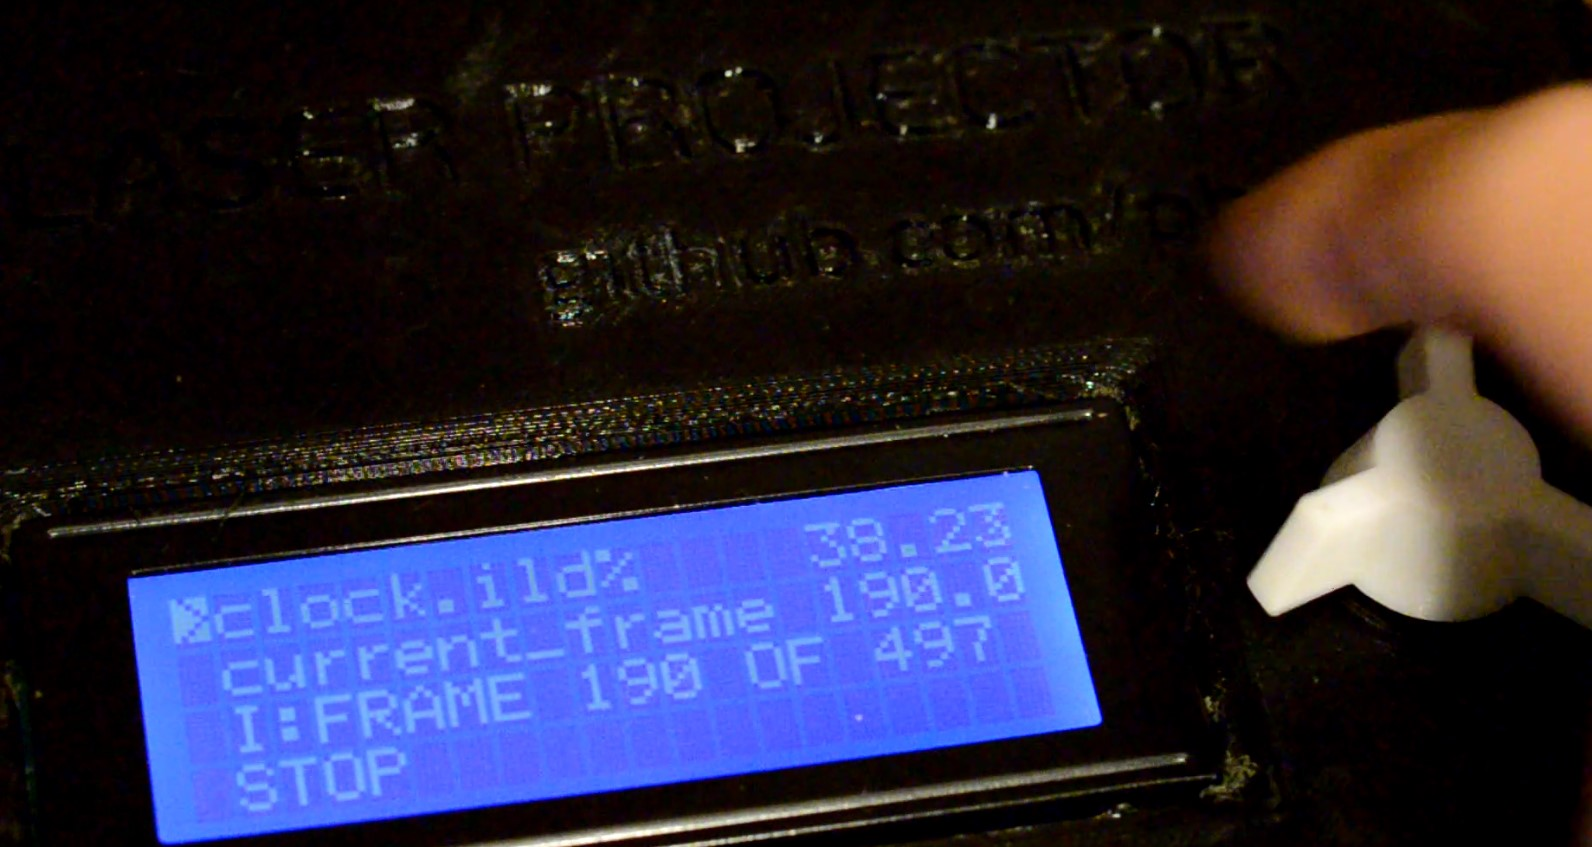
\includegraphics[width=1\textwidth]{img/ui_lcd_main.jpg}
    \caption{\label{fig:uilcdmain} Úvodní obrazovka menu na LCD; Zobrazuje se odshora: procentuální poměr počtu zobrazených snímků vůči celkovému počtu snímků v projekci, číslo aktuálního snímku v sekvenci, poslední přijatá zpráva od programu lasershow a tlačítko k zastavení projekce. Napravo od obrazovky je vidět rotační enkodér se kterým uživatel interaguje.}
\end{figure}
\begin{figure}[H]
    \centering
    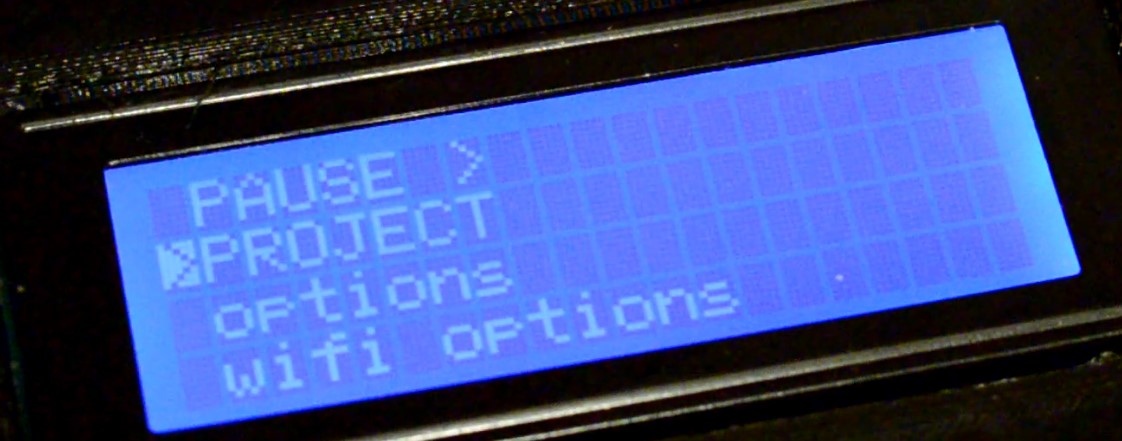
\includegraphics[width=1\textwidth]{img/ui_lcd_second.jpg}
    \caption{\label{fig:uilcdsec} Pokračování úvodní obrazovky menu na LCD; Odshora je vidět tlačítko k zastavení projekce v čase, sekundární menu pro výběr souboru, sekundární menu pro nastavení projekce a sekundární menu pro nastavení WiFi připojení.}
\end{figure}
\begin{figure}[H]
    \centering
    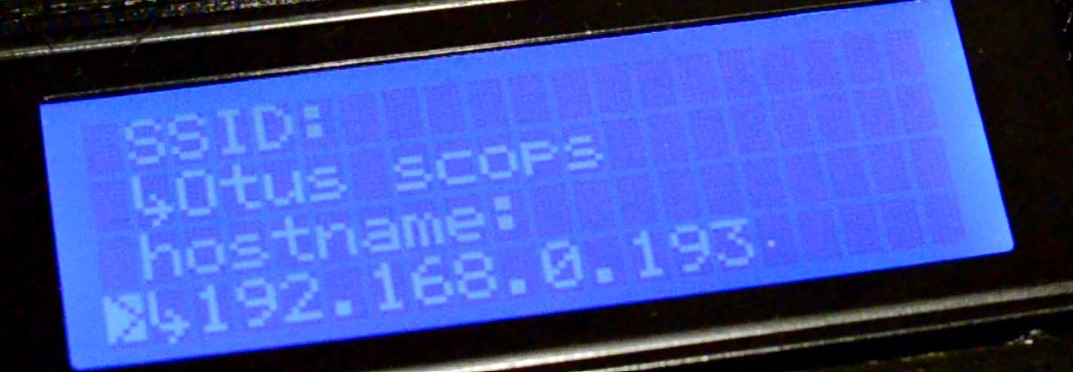
\includegraphics[width=1\textwidth]{img/ui_lcd_wifi.jpg}
    \caption{\label{fig:uilcdwifi} Sekundární menu pro nastavení WiFi připojení na LCD}
\end{figure}

\subsection{Využité knihovny}
\subsubsection{wPi\_soft\_lcd}
Hlavní využitou knihovnou je~wPi\_soft\_lcd~\cite{wpi-lcd}. Tato knihovna umožňuje jednoduchou komunikaci s~LCD prostřednictvím I$^{2}$C převodníku. Její použití je~vidět v~ukázce kódu v~příloze~\ref{list:soft_lcd}.

% Mezi nejdůležitější funkce této knihovny, které používám ve~svém kódu patří:
% \begin{itemize}
%     \item \mintinline{cpp}{lcd_t *lcd_create(int scl, int~sda, int~addr, int~lines)} --- Tato funkce inicializuje komunikaci s~I$^{2}$C převodníkem. Je~nutné ji~zavolat před jiným použitím knihovny.
%           Příjmá čísla pinů I$^{2}$C sběrnice, na~které je~připojený displej, dále příjmá I$^{2}$C adresu převodníku a~počet řádků displeje. Funkce vrací pointer na~nově vytvořenou strukturu typu \mintinline{cpp}{lcd_t}, který je~potřeba k~volání dalších funkcí knihovny. Jestliže se~nepodaří inicializovat knihovnu, vrací hodnotu \mintinline{cpp}{NULL}.
%     \item \mintinline{cpp}{void lcd_printf(lcd_t *lcd, const char* format, ... )} --- K~vypsání textu na~LCD~využívám tuto funkci. Příjmá pointer vrácený funkcí \mintinline{cpp}{lcd_create}, formátovací řetězec a~případně další argumenty stejně, jako známá funkce \mintinline{cpp}{printf} ze~standartní knihovny programovacího jazyka C.
%     \item \mintinline{cpp}{void lcd_clear (lcd_t *lcd)} --- Funkce při jejím zavolání vymaže všechen text zobrazený na~LCD. Příjmá pointer funkcí \mintinline{cpp}{lcd_create}.
%     \item \mintinline{cpp}{void lcd_pos(lcd_t *lcd, int~row, int~col)} --- Touto funkcí je~možno nastavit pozici virtuálního kurzoru, od~kterého začne vypisovat funkce \mintinline{cpp}{lcd_printf}. Příjmá pointer funkcí \mintinline{cpp}{lcd_create}, číslo řádku a~číslo sloupce požadované pozice kurzoru. Obě čísla jsou počítaná od~nuly.
%     \item \mintinline{cpp}{void lcd_backlight_dim (lcd_t *lcd, float intensity)} --- Funkce, která nastaví střídu PWM~signálu na~GPIO pinu 18 a~tím reguluje jas~podsvícení LCD. Příjmá pointed vrácený funkcí \mintinline{cpp}{lcd_create} a~desetinné číslo od~0 do~1, značící požadovanou intenzitu podsvícení.
%     \item \mintinline{cpp}{void lcd_create_char(lcd_t *lcd, int~n, char *data)} --- Touto funkcí je~možné definovat vlastní znaky, které se~zobrazí na~LCD. Příjmá pointer vrácený funkcí \mintinline{cpp}{lcd_create}, číslo znaku, který má být definován a~pole 8 bytů, které reprezentuje vlastní znak.
%     \item \mintinline{cpp}{}
%     \item \mintinline{cpp}{}
%     \item \mintinline{cpp}{}
%     \item \mintinline{cpp}{}
% \end{itemize}

\subsubsection{wiringPi}
Předchozí popsaná knihovna pro~posílání signálu I$^{2}$C sběrnicí používá knihovnu wiringPi, která umožňuje ovládání GPIO pinů. Abych nepřidával do~jednoho programu dvě knihovny interagující s~hardwarem, stejnou knihovnu využívám i~pro čtení dat~z enkodéru. Její využití k~detekci změn na~pinech enkodéru je~vidět na~ukázce kódu v~příloze~\ref{list:wiringpi}.

Je nepraktické využívat ve~dvou programech jinou knihovnu na~interakci s~hardwarem, proto v~budoucnu budou knihovna wPi\_soft\_lcd a~celý tento program přepsány tak, aby~využívaly modernější knihovnu pigpio popsanou v~kapitole~\ref{sec:ls_pigpio} stejně jako program lasershow.

% \begin{itemize}
% \item \mintinline{cpp}{void pinMode (int pin, int~mode)} --- Funkce, která pro~GPIO pin~z argumentu \mintinline{cpp}{pin} nastaví mód z~argumentu \mintinline{cpp}{mode}. Jako argument \mintinline{cpp}{mode} používám hodnotu \mintinline{cpp}{INPUT}, která pin~zaregistruje pro~vstup.
% \item \mintinline{cpp}{void pullUpDnControl (int pin, int~pud)} Funkce připojí na~pin~\mintinline{cpp}{pin} pull-up nebo pull-down rezistor podle argumentu \mintinline{cpp}{pud}. Jako argument \mintinline{cpp}{pud} používám hodnotu \mintinline{cpp}{PUD_UP}, která k~pinu připojí pull-up rezistor.
% \item \mintinline{cpp}{int wiringPiISR (int pin, int~mode, void (*function)(void))} --- Tato funkce nastaví přerušení na~pin~\mintinline{cpp}{pin}. Tak, aby~při změně hodnoty na~tomto pinu byla zavolána tzv. callback funkce z~argumentu \mintinline{cpp}{function}. Argument \mintinline{cpp}{mode} úrčuje, jestli je~funkce zavolána pouze při tzv. rising edge, tzv. falling edge, nebo při obou. Já v~tomto argumentu používám hodnotu \mintinline{cpp}{INT_EDGE_BOTH}.
% \end{itemize}

\subsubsection{cppzmq}
Samozřejmě program také využívá knihovnu cppzmq~\cite{cppzmq} popsanou v~kapitole~\ref{sec:ls_cppzmq}. Program ji~používá podobně jako program lasershow, ne~však stejně.

Největším rozdílem je, že místo funkce \mintinline{cpp}{void zmq::socket_t::bind} používá funkci \mintinline{cpp}{void zmq::socket_t::connect(const char *addr_)}.
Funkci \mintinline{cpp}{bind} je~totiž potřeba zavolat přesně jednou pro~každý socket.
Jestliže ji~už pro~sockety zavolal program lasershow, popřípadě wifi\_manager a~socket tedy už je~registrovaný k~danému portu, je~třeba zavolat funkci \mintinline{cpp}{connect}.

Dále samozřejmě stejně jako všechny frontendové programy do~vstupního socketu zprávy posílá a~z výstupního socketu zprávy čte. Celková ukázka využití knihovny frontendovým programem v~jazyce C++ je~v ukázce kódu v~příloze~\ref{list:zmq_c_cpp}.

\subsection{Struktura programu}
Program začne inicializací komunikace s~LCD.
Poté pokračuje registrací interruptů na~pinech, ke~kterým je~připojen enkodér. A~následně se~připojí k~socketům aplikací lasershow a~wifi\_manager.

V další části programu je~definováno samotné menu. To~má podobu struktury \mintinline{cpp}{menu_option}. V~ukázce kódu v~příloze~\ref{list:menu_option} je~vidět, jak~je tato struktura dufinována.

Díky ní je~možné definovat menu poměrně jednoduchým způsobem. Zkrácený příklad je~v ukázce kódu v~příloze~\ref{list:menu_def}.

Následuje nekonečný cyklus, ve~kterém program příjmá zprávy od~programů lasershow a~wifi\_manager a~volá funkci \mintinline{cpp}{bool menu_interact(lcd_t *lcd, zmq::socket_t &command_sender, menu_option &parent_menu_option, bool redraw = 0)}, která rekurzivně prochází menu následujícím způsobem.
Vždy, pokud má atribut \\
\mintinline{cpp}{parent_menu_option.nest_option_active} hodnotu true a~atribut \mintinline{cpp}{style} objektu \mintinline{cpp}{parent_menu_option.nested_menu_options[nest_selected]} je~roven \mintinline{cpp}{NESTED_MENU}, zavolá sebe samou, ale~jako argument \mintinline{cpp}{parent_menu_option} použije právě objekt \\
\mintinline{cpp}{parent_menu_option.nested_menu_options[nest_selected]}.
\fxnote{TODO: před odevzdanim osetrit line breaks tady}
Jakmile takto najde zrovna aktivní položku menu, přečte proměnnou, kde~je~uložená relativní pozice enkodéru oproti poslednímu čtení a~dle této proměnné se~změní proměnnou \mintinline{cpp}{parent_menu_option.nest_selected}.

Pokud narazí na~aktivní položku menu, jejíž atribut \mintinline{cpp}{style} je~roven \mintinline{cpp}{VALUE}, chování funkce se~lehce změní. V~takovém případě se~změní hodnota, kterou tato položka menu reprezentuje. Ta~je~uložena v~atributu \mintinline{cpp}{value} právě vybrané položky.

\section{web\_ui}

Narozdíl od~předchozích dvou zmiňovaných programů je~program web\_ui psaný v~jazyce javascript, ten~nepatří mezi nejrychlejší, ale~díky runtime Node.js a~knihovnám http a~formidable v~něm bylo časově nenáročné vytořit http web~server.

Tento server běží na~portu 3000 a~je~dostupný z~lokální sítě (tzn. přímo z\~Raspberry Pi~na~adrese http://localhost:3000 nebo z~jakéhokoliv zařízení na~stejné lokální síti na~IP~adrese RPi).
Program je~využíván pro~jednoduchou interakci s~uživatelem.
Ten může pomocí webového prohlížeče ovládat laserový projektor pár kliknutími nebo zadávat vlastní příkazy klávesnicí.

Ve webovém prostředí jsou zatím konzole pro~ssh přístup k~Raspberry Pi~a~pro komunikaci s~programy wifi\_manager a~lasershow.
Také je~v~něm formulář, kde~si~uživatel může jednoduše vybrat soubor k~projekci.
V něm se~mu~zobrazí soubory už uložené ve~složce pro~ně určené. Dále se~ve~webovém prostředí nachází formulář, kterým uživatel do~této složky může soubor nahrát. Soubory může nahrávat ve~formátech .svg a~.ild.
Aktuální stav webového rozhraní je~vidět na~obrázcích~\ref{fig:uisshfile} a~\ref{fig:uiwebsettings}.

\begin{figure}[ht]
    \centering
    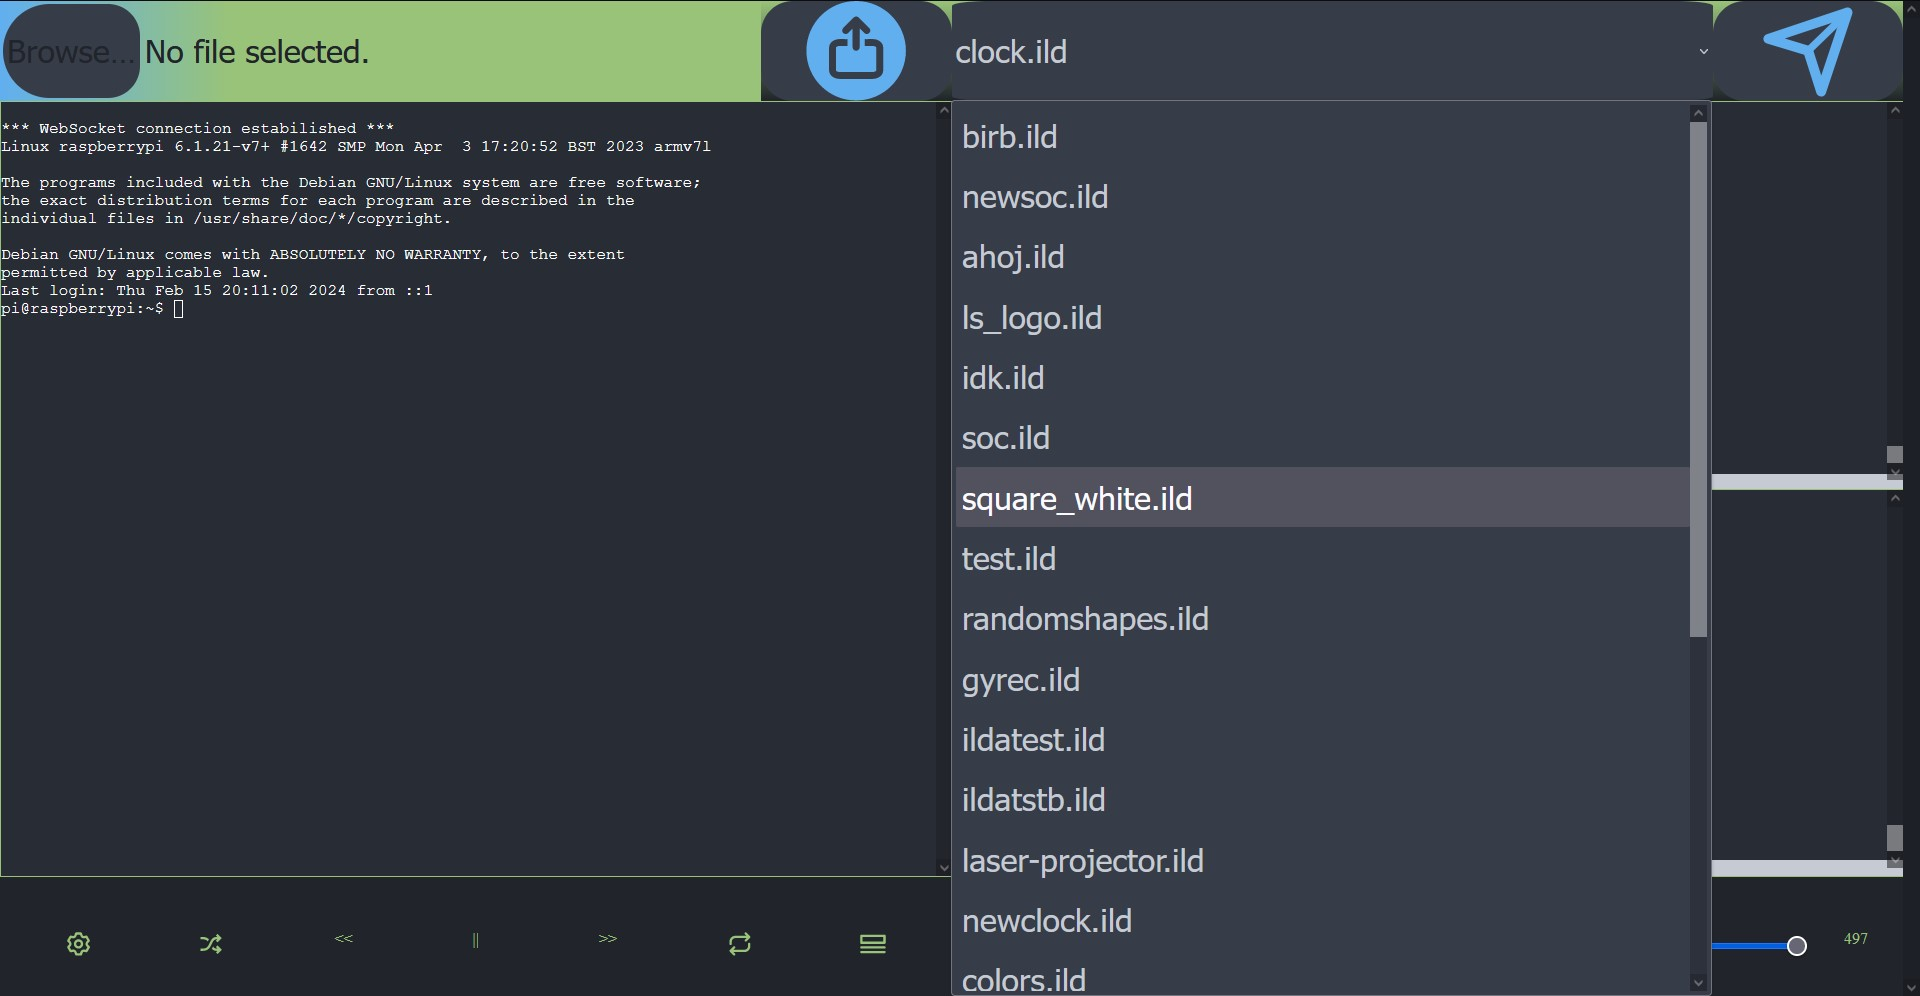
\includegraphics[width=1\textwidth]{img/ui_ssh-file.jpg}
    \caption{\label{fig:uisshfile} Webové rozhraní; Napravo si uživatel vybírá soubor k projekci, nalevo je vidět odshora: formulář pro nahrání souboru, ssh konzole a základní ovládací prvky.}
\end{figure}

\begin{figure}[ht]
    \centering
    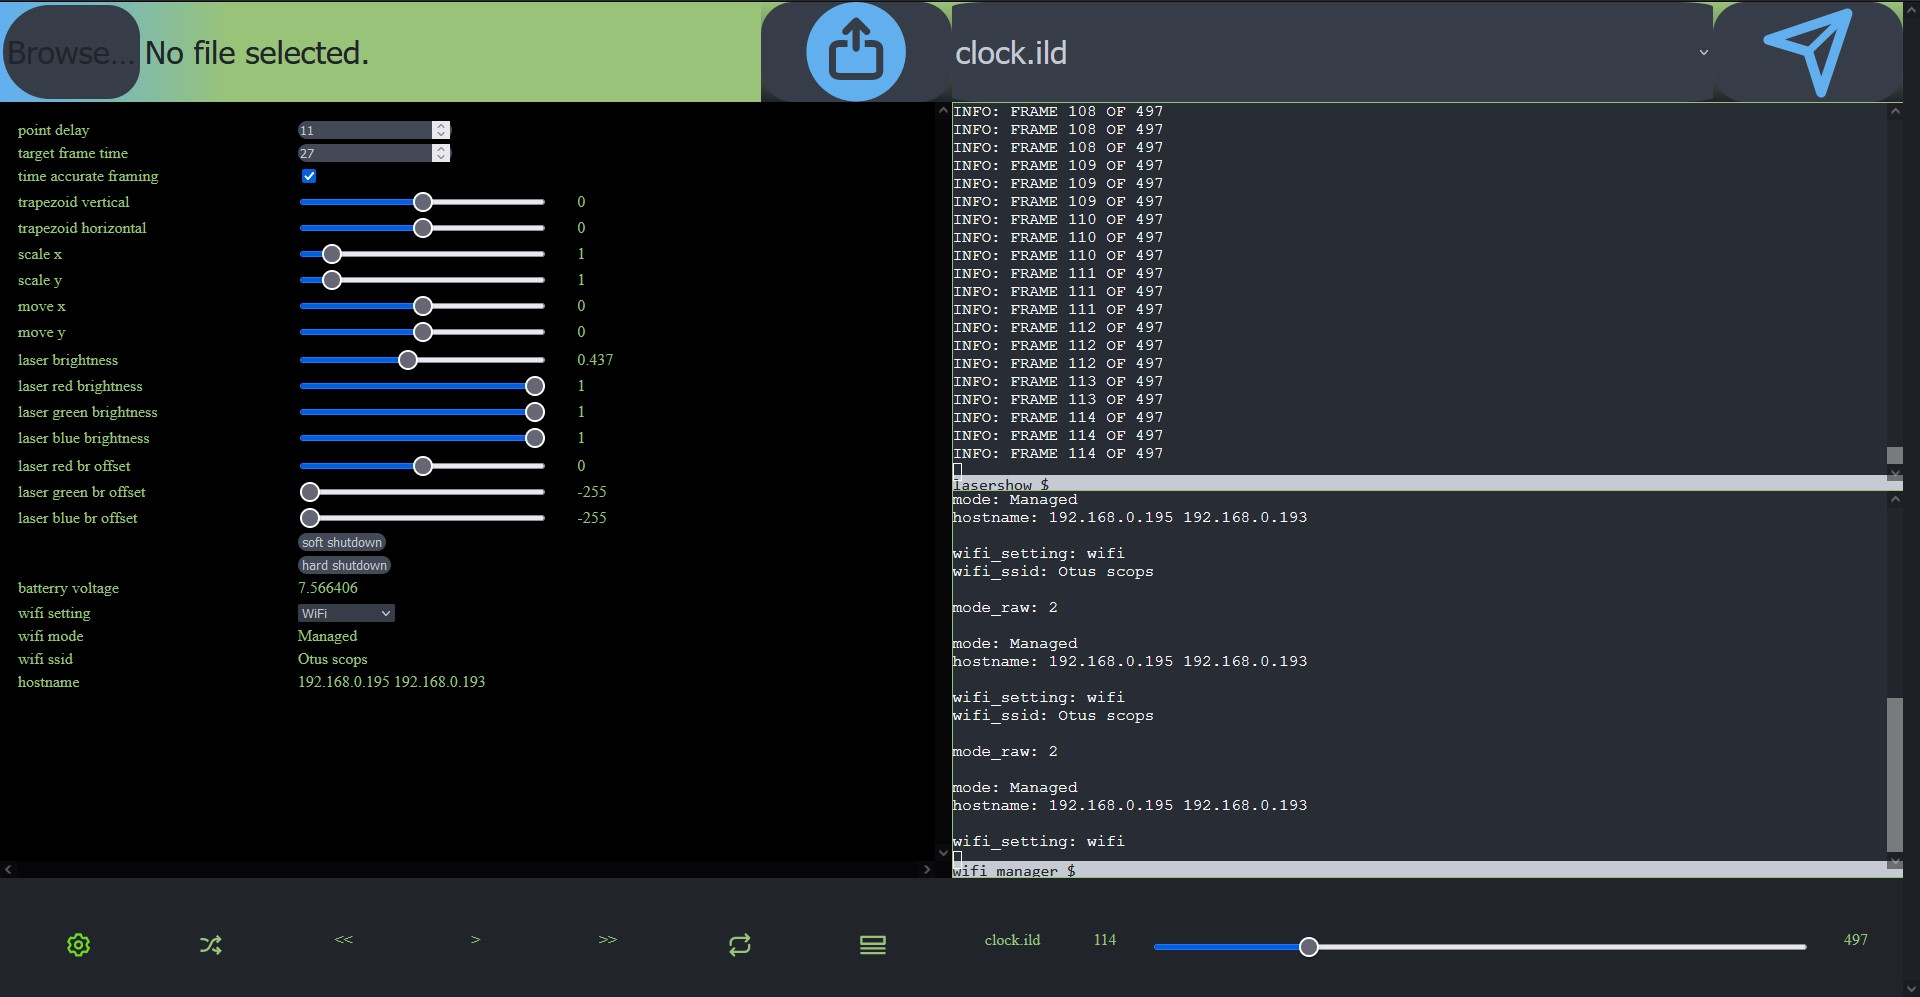
\includegraphics[width=1\textwidth]{img/ui_web_settings.jpg}
    \caption{\label{fig:uiwebsettings} Webové rozhraní; Nalevo jsou vidět nastavení a informace o stavu baterie a WiFi připojení. To vše bylo zobrazeno po kliknutí na ikonku ozubeného kola v levém dolním rohu. Barva této ikonky je nyní saturovanější. Napravo je vidět odshora: formulář pro výběr souboru k projekci, konzole programu lasershow, konzole programu wifi\_manager a úplně dole název a průběh aktuálně vykreslovaného souboru.}
\end{figure}

V blízké budoucnosti do~prostředí přibudou prvky, které mohou ovládat frontu, nastavení programů lasershow a~wifi\_manager. Později by~měla přibýt funkce kreslení v~prohlížeči, kdy~uživatel bude moct v~prohlížeči nakreslit požadovaný tvar a~projektor ho~už v~průběhu kreslení bude promítat. Tato funkce by~měla v~budoucnu být propojena s~kamerou připojenou na~Raspberry Pi. V~tu~chvíli uživatel bude mít možnost v~prohlížeči kreslit do~obrazu reálného světa.

\subsection{Využité knihovny}
\subsubsection{Http}
Knihovna http je~využita k~jednoduchému vytvoření interaktivního http serveru, ke~kterému se~uživatel může připojit ze~svého prohlížeče. Příklad takového serveru je~vidět v~ukázce kódu v~příloze~\ref{list:http}.
    
\subsubsection{Zeromq.js, ssh2, socket.io a~xterm.js}
Http server tedy pošle prohlížeči uživatele kód, který v~tomto prohlížeči běží. Poté je~knihovna socket.io využita ke~komunikaci mezi kódem běžícím v~prohlížeči uživatele (klientem) a~kódem běžícím na~Raspberry Pi~(serverem).
Společně s~knihovnou zeromq.js umožňují tomuto programu fungovat jako prostředník mezi klientem a~backendovými programy. Díky knihovně ssh2 také tímto spojením je~možné přímo z~prohlížeče psát do~příkazového řádku.

Knihovna xterm.js běžící v~kódu klienta je~využita k~dosažení interaktivity a~vzhledu konzolí, které se~uživateli ve~webovém rozhraní zobrazují.

V ukázkách kódu v~přílohách~\ref{list:socketio_s} a~\ref{list:socketio_c} je~vidět, jak~server předává klientovi data od~backendových programů a~jak je~klient uživateli vykresluje.

% \subsubsection{}
% Stejně jako program UI~za~pomoci knihovny ZeroMQ tento program odebírá z~výstupního socketu zprávy o~průběhu vykreslování od~programu lasershow a~odesílá mu~pokyny uživatele na~vstupní socket.

% \inputminted[frame=lines,fontsize=\footnotesize{}, linenos, breaklines]{js}{code_examples/zmq_client.js}

\section{discord bot}

Posledním programem, který by~měl být využíván k~interakci s~uživatelem je~discord\_bot. Ten~bude naprogramován a~uveden do~provozu v~blízké budoucnosti.

Měl by~sloužit k~interakci s~uživatelem v~chattovací aplikaci discord. Bude~také psaný v~jazyce javascript v~runtime Node.js, stejně jako předchozí programy se~přihlásí k~socketům knihovnou zmq, ale~na~rozdíl od~nich tento program bude moct interagovat s~uživatelem přes internet, ať už je~kdekoliv na~světě.

Pomocí knihovny discord.js se~přihlásí k~předem vytvořenému bot~účtu, který může na~předem vytvořeném discord serveru čekat na~zprávy od~uživatele, ty~posílat do~vstupního socketu a~posílat uživateli zpětnou vazbu, kterou příjme z~výstupního socketu.
